\chapter{Конструкторская часть}
В данном разделе будут представлены математические основы для реализации алгоритма обратной трассировки лучей, схемы данного алгоритма и необходимых подпрограмм и обоснование используемых типов и структур данных.

\section{Математические основы для реализации алгоритма обратной трассировки лучей}
\subsection{Поиск пересечения луча со сферой}
Использован геометрический подход. Основные обозначения представлены для наглядности на рис. \ref{img:sphere}.

\begin{figure}[h!]
    \centering
    \includegraphics[width=0.8\linewidth]{sphere.pdf}
    \caption{Геометрический подход при поиске пересечения луча со сферой}
    \label{img:sphere}
\end{figure}

Нужно произвести следующие действия (все обозначения соответствуют представленным на рис. \ref{img:sphere}, индекс $i$ используется для значений, связанных с точкой пересечения луча и сферы, $c$~---~с точкой центра сферы):
\begin{enumerate}[label={\arabic*)}]
	\item Проверка, лежит ли начало луча внутри сферы. Для этого вычисляется длина вектора $OC$: $OC = S_c - R_0$. Если $OC < R$, то начало луча лежит внутри сферы.
	\item Нахождение ближайшей к центру сферы точки луча, расстояние до которой от центра обозначается как $D$. Расстояние до этой точки от начала луча обозначается как $t_{ca}$. Тогда $t_{ca} = OC \cdot dir$ (равно проекции $OC$ на направление луча), где $dir$~---~это директриса луча. \\ Теперь если $t_{ca} < 0$ и $R_0$ вне сферы, то луч не пересекает данную сферу. Иначе выполняются следующие действия.
	\item Нахождение расстояния от ближайшей к центру точки луча до точки пересечения со сферой. Вычисляется $D^2 = OC^2 - t_{ca}^2$ по теореме Пифагора. Тогда $t_{hc}^2 = R^2 - D^2 = R^2 - (OC^2 - t_{ca}^2)$ также по теореме Пифагора. \\ Теперь если $t_{hc}^2 < 0$, то луч не пересекает данную сферу. Иначе выполняются следующие действия.
	\item Вычисление расстояния от начала луча до точки пересечения. Если $R_0$ внутри сферы, то используется формула $t = t_{ca} + t_{hc}$, иначе используется формула $t = t_{ca} - t_{hc}$. 
	\item Вычисление координат точки пересечения луча со сферой. Используется формула $R(t) = R_0 + R_dt$ (в параметрической форме) или $(x_i, y_i, z_i) = (x_0 + x_dt, y_0 + y_dt, z_0 + z_dt)$ (в координатах).
\end{enumerate}

Также, удобно сразу вычислить нормаль к точке пересечения при помощи формулы:
\begin{equation}
	n = \begin{pmatrix}
		\frac{x_i - x_c}{R}, & \frac{y_i - y_c}{R}, & \frac{z_i - z_c}{R}
	\end{pmatrix}^{T}.
\end{equation}

\subsection{Поиск пересечения луча с многогранником}
Для поиска пересечения луча с многогранником необходимо осуществить поиск пересечения луча с каждой его гранью (многоугольником). Данная задача рассмотрена ниже.

Однако, есть ситуации, когда можно сразу понять, пересекается ли многогранник заданным лучом, выполнив менее трудозатратные вычисления. Для этого перед проверкой всех полигонов многогранника проверяется пересечение лучом сферической оболочки, в которую вписан многогранник, по вышеописанному алгоритму. На рис. \ref{img:sphere-cover} изображена сферическая оболочка для четырёхугольной пирамиды.

\begin{figure}[h!]
    \centering
    \includegraphics[width=0.35\linewidth]{sphere-cover.pdf}
    \caption{Сферическая оболочка для четырёхугольной пирамиды}
    \label{img:sphere-cover}
\end{figure}

\newpage

\subsection{Поиск пересечения луча с полигоном (многоугольником)}
Любой луч представим параметрическим уравнением вида $R(t) = R_0 + R_dt$. Любая плоскость представима в виде $ax + by + cz + d = 0$. Для данной плоскости: \begin{itemize}
	\item $a^2 + b^2 + c^2 = 1$;
	\item $n = \begin{pmatrix}
		a, & b, & c \end{pmatrix}^{T}$;
	\item расстояние от данной плоскости до точки $(0,0,0)$ равняется $-d$.
\end{itemize}

Уравнение луча можно представить в виде плоскости и разрешить относительно параметра $t$:
\begin{equation}
	t = \frac{-(ax_0 + by_0 + cz_0 + d)}{ax_d + by_d + cz_d}.
\end{equation}

Тогда если $ax_d + by_d + cz_d = 0$, то луч параллелен плоскости, и пересечения точно нет. Если $t < 0$, то пересечение происходит с прямой, на которой лежит луч, а не с самим лучом. Иначе, существует пересечение луча с заданной плоскостью в точке $(x_i, y_i, z_i) = (x_0 + x_dt, y_0 + y_dt, z_0 + z_dt)$. 

Теперь необходимо проверить, принадлежит ли точка пересечения с плоскостью многоугольнику. Для этого применяется самый распространённый тест: проверяются последовательно знаки векторных произведений каждой стороны полигона на вектор, соединяющий начало текущей стороны и точку пересечения. Если какое-либо векторное произведение нулевое, значит точка лежит на стороне полигона. Если знаки всех векторных произведений совпадают, то точка принадлежит полигону, иначе она находится вне полигона.

На рис. \ref{img:inside} изображены возможные ситуации при данной проверке.

\newpage

\begin{figure}[h!]
    \centering
    \includegraphics[width=0.3\linewidth]{inside.pdf}
    \caption{Возможные ситуации при проверке принадлежности точки полигону}
    \label{img:inside}
\end{figure}

Векторные произведения $AQ \times AB$ и $BQ \times BC$, например, будут иметь разные знаки, так как точка $Q$ лежит вне полигона. Векторные произведения $AP \times AB$ и $BP \times BC$ будут иметь одинаковые знаки (как и $AP \times AC$), так как точка $P$ лежит внутри полигона. При рассмторении точки $O$ одно из векторных произведений будет нулевым, так как она лежит на стороне полигона.

\subsection{Поиск коэффициентов уравнения плоскости полигона и вектора нормали}
Если известны 3 точки, принадлежащие плоскости, то можно найти коэффициенты уравнения плоскости, приведя следующую запись к виду уравнения плоскости:
\begin{equation}
	\begin{vmatrix}
		x - x_0 & x_1 - x_0 & x_2 - x_0 \\
		y - y_0 & y_1 - y_0 & y_2 - y_0 \\
		z - z_0 & z_1 - z_0 & z_2 - z_0
	\end{vmatrix} = 0.
\end{equation}

Будут получены следующие уравнения для коэффициентов:
\begin{equation}
	A = (y_1 - y_0)(z_2 - z_0) - (y_2 - y_0)(z_1 - z_0),
\end{equation}
\begin{equation}
	B = (x_1 - x_0)(z_2 - z_0) - (x_2 - x_0)(z_1 - z_0),
\end{equation}
\begin{equation}
	C = (x_1 - x_0)(y_2 - y_0) - (x_2 - x_0)(y_1 - y_0),
\end{equation}
\begin{equation}
	D = -Ax_0 + By_0 - Cz_0.
\end{equation}

Далее следует подставить в уравнение с полученными коэффициентами точку, координаты которой соответствуют усреднённому значению координат всех вершин данного полигона. Если значение положительное, то коэффициенты следует домножить на -1, так как осуществляется поиск внешней нормали.
Формально используются координаты векторов, составляющих стороны полигона. Иллюстрация представлена на рис. \ref{img:norm}.\\

\begin{figure}[h!]
    \centering
    \includegraphics[width=0.3\linewidth]{norm.pdf}
    \caption{Выбор векторов для поиска вектора нормали к полигону}
    \label{img:norm}
\end{figure}

Тогда вектор нормали к данному полигону можно представить как
\begin{equation}
	n = \begin{pmatrix} A, & B, & C
 \end{pmatrix}^{T},
\end{equation}
где $A, B, C$~---~коэффициенты уравнения плоскости заданного полигона.

\subsection{Определение направлений отражённого и преломлённого лучей}
Для алгоритма обратной трассировки лучей необходимо вычислять направления отражённого и преломлённого лучей. Пусть $A$~---~направление падающего луча, $B$~---~направление отражённого луча, $C$~---~направление преломлённого луча, а $N$~---~нормаль к поверхности. Луч $A$ можно разбить на два слагаемых: $A_p$~---~вектор, перпендикулярный нормали, и  $A_n$~---~вектор, параллельный нормали. На рис. \ref{img:angle} изображены направления данных лучей и приведены используемые ниже обозначения, причём все вектора нормализованы.

\begin{figure}[h!]
    \centering
    \includegraphics[width=0.31\linewidth]{angle.pdf}
    \caption{Направления отражённого и преломлённого лучей}
    \label{img:angle}
\end{figure}

%Все три вектора ($A, B, N$) лежат в одной плоскости, значит можно выразить один из них через два других: $B = a \cdot -A + b \cdot N$. Учитывая нормализованность векторов можем записать:
%\begin{equation}
%	(-A, N) = \cos(1),
%\end{equation}
%\begin{equation}
%	(N, B) = \cos(2).
%\end{equation}
%
%Учитывается равенство углом падания и отражения:
%\begin{equation}
%	(-A, N) = (N, B) = (N, a \cdot -A + b \cdot N) = a \cdot (N, -A) + b.
%\end{equation}
%
%Пусть $a = -1$. Тогда $B = 2 \cdot (N, -A) \cdot N + A$.

По свойству скалярного произведения $A_n = N(N \cdot (-A))$ и  $A_p = -A - A_n = -A + N(N \cdot A)$.
Отражённый луч можно выразить через разность этих векторов $B = A - 2 N(N \cdot A)$.

Падающий, преломлённый луч и нормаль к поверхности лежат в одной плоскости. Пусть $ \mu_i$ -- показатели преломления сред, причём $i = \overline{1,2}$. 
Применяя закон Снеллиуса, параметры преломлённого луча можно вычислить по формуле
\begin{equation}
\begin{aligned}
C = \frac{\mu_1}{\mu_2}A + ( \frac{\mu_1}{\mu_2}\cos(\alpha_1) - \cos(\alpha_3))N ,
\end{aligned}
\end{equation} 
где $cos(\alpha_3) = \sqrt{1 - (\frac{\mu_1}{\mu_2})^2(1 - cos(\alpha_1))^2}$.

\section{Разработка алгоритма обратной трассировки лучей}
На рисунке \ref{img:raytrace} представлена схема алгоритма обратной трассировки лучей.

\begin{figure}[h!]
    \centering
    \includegraphics[width=0.9\linewidth]{raytrace-2.pdf}
    \caption{Схема алгоритма обратной трассировки лучей}
    \label{img:raytrace}
\end{figure}

\newpage

На рисунке \ref{img:sceneIntersect} представлена схема подпрограммы поиска ближайшего пересечения луча с объектом сцены.

\begin{figure}[h!]
    \centering
    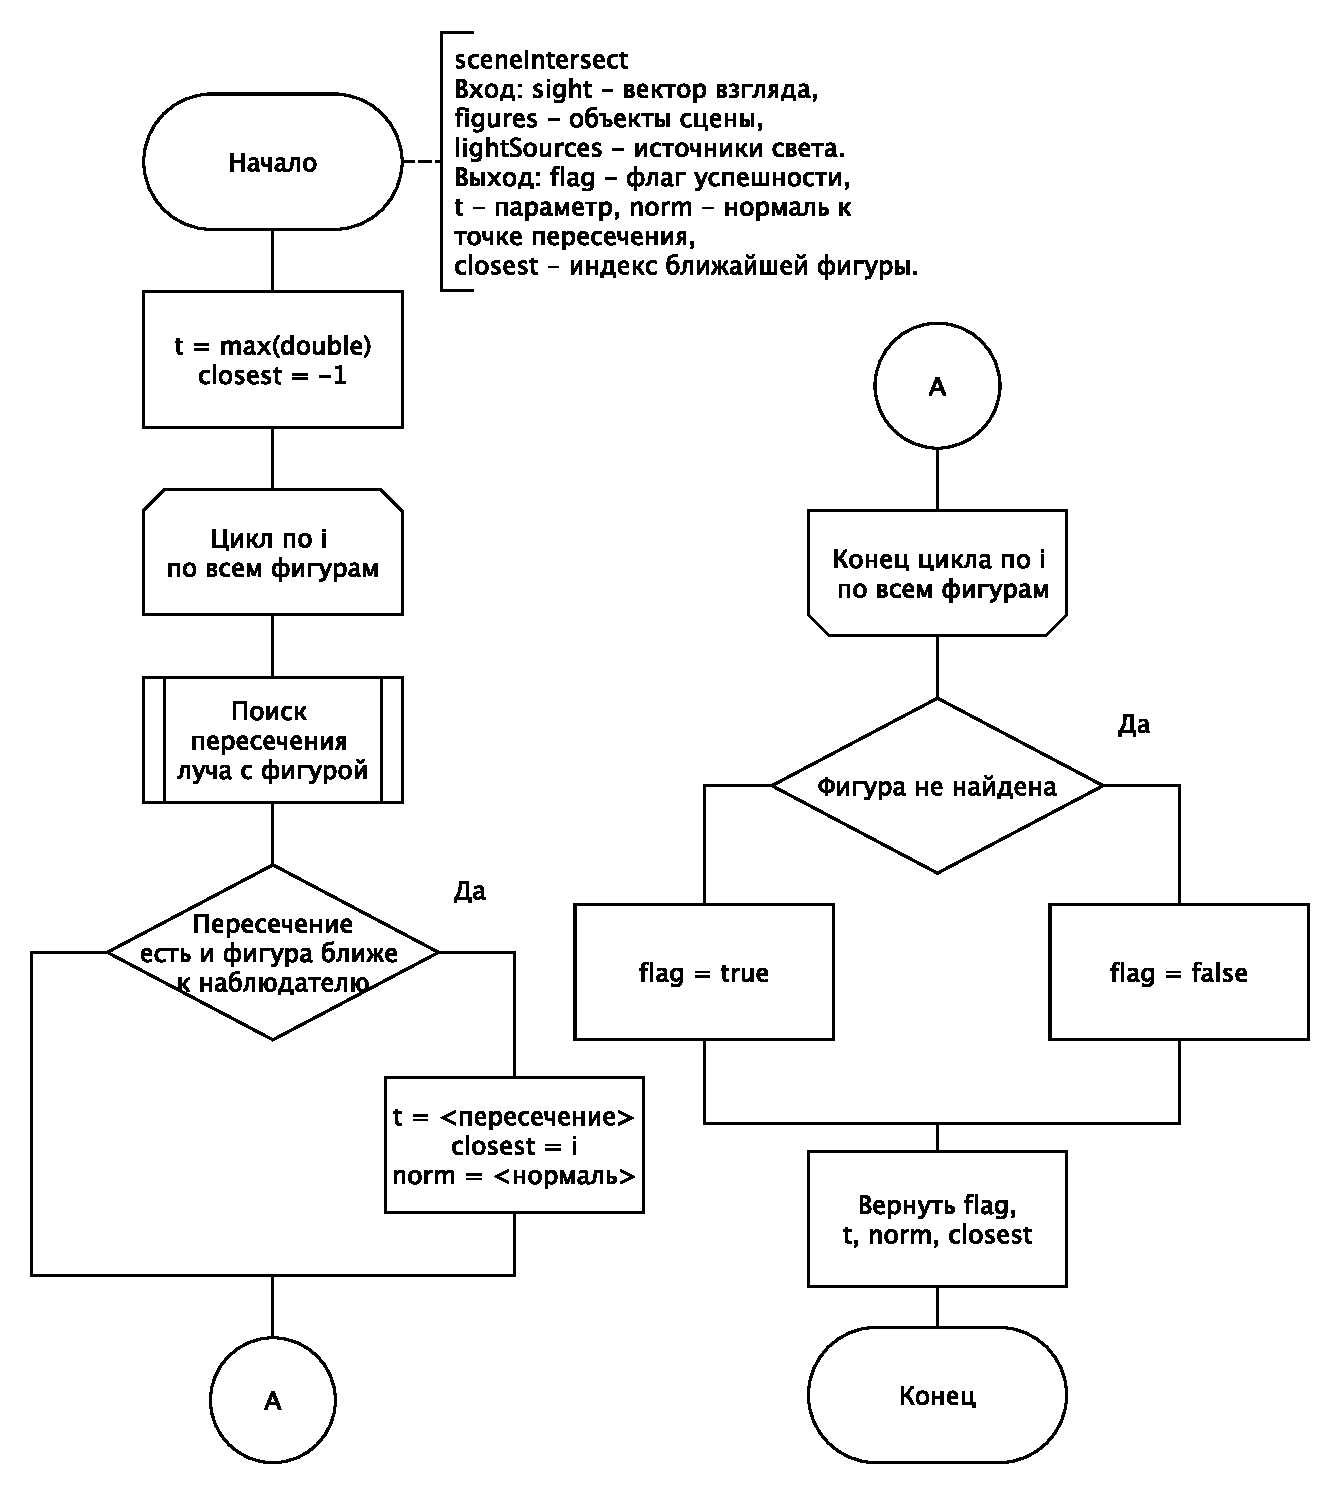
\includegraphics[width=1\linewidth]{sceneIntersect.pdf}
    \caption{Схема подпрограммы поиска ближайшего пересечения луча с объектом сцены}
    \label{img:sceneIntersect}
\end{figure}

\newpage

На рисунке \ref{img:rayPolygon} представлена схема подпрограммы поиска точки пересечения луча с многогранником. На рисунке \ref{img:rayGran} представлена схема подпрограммы поиска точки пересечения луча с треугольным полигоном.

\begin{figure}[h!]
    \centering
    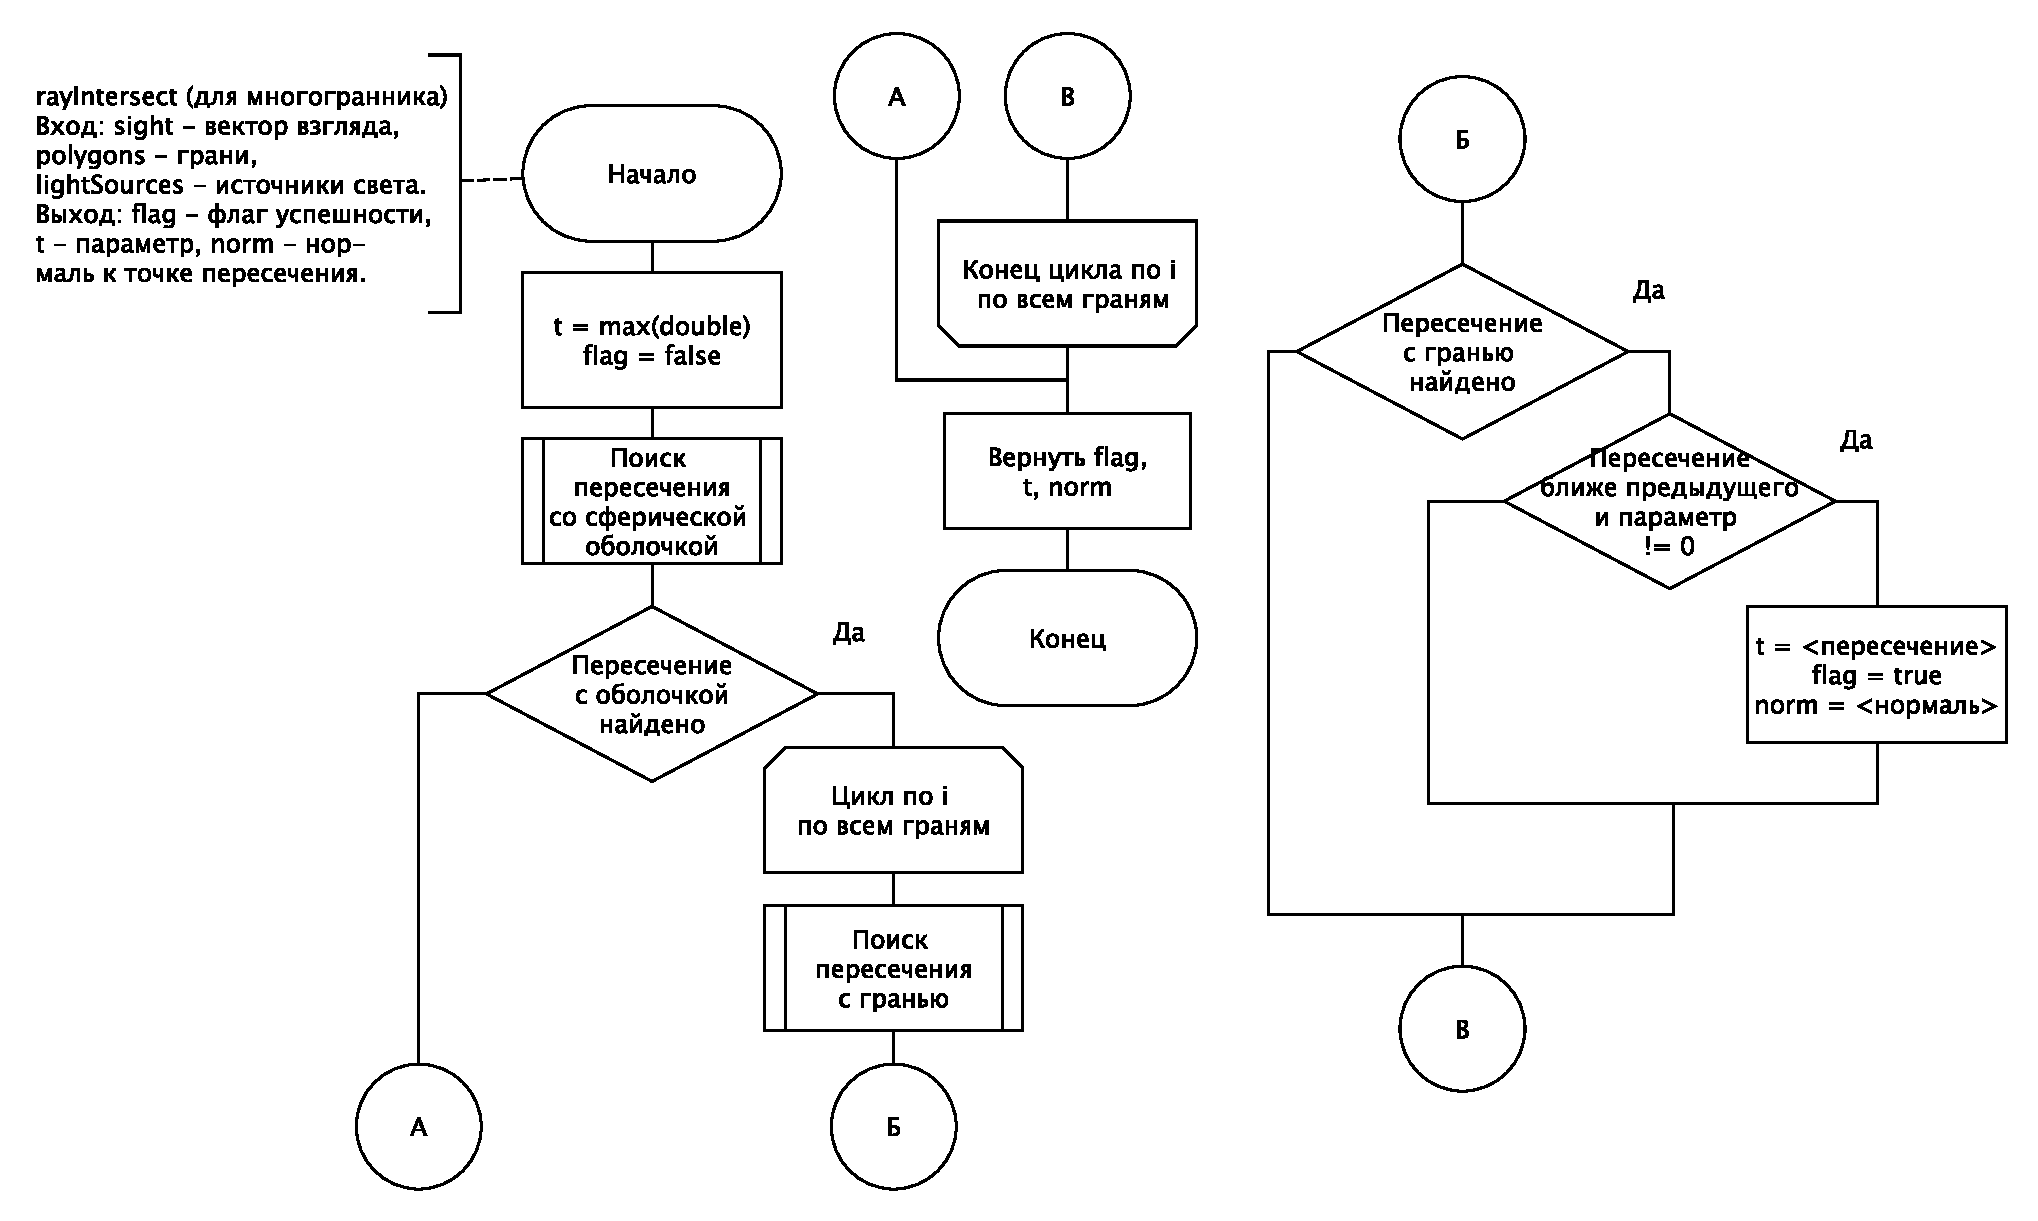
\includegraphics[width=0.75\linewidth]{rayPolygon.pdf}
    \caption{Схема подпрограммы поиска точки пересечения луча с многогранником}
    \label{img:rayPolygon}
\end{figure}

\begin{figure}[h!]
    \centering
    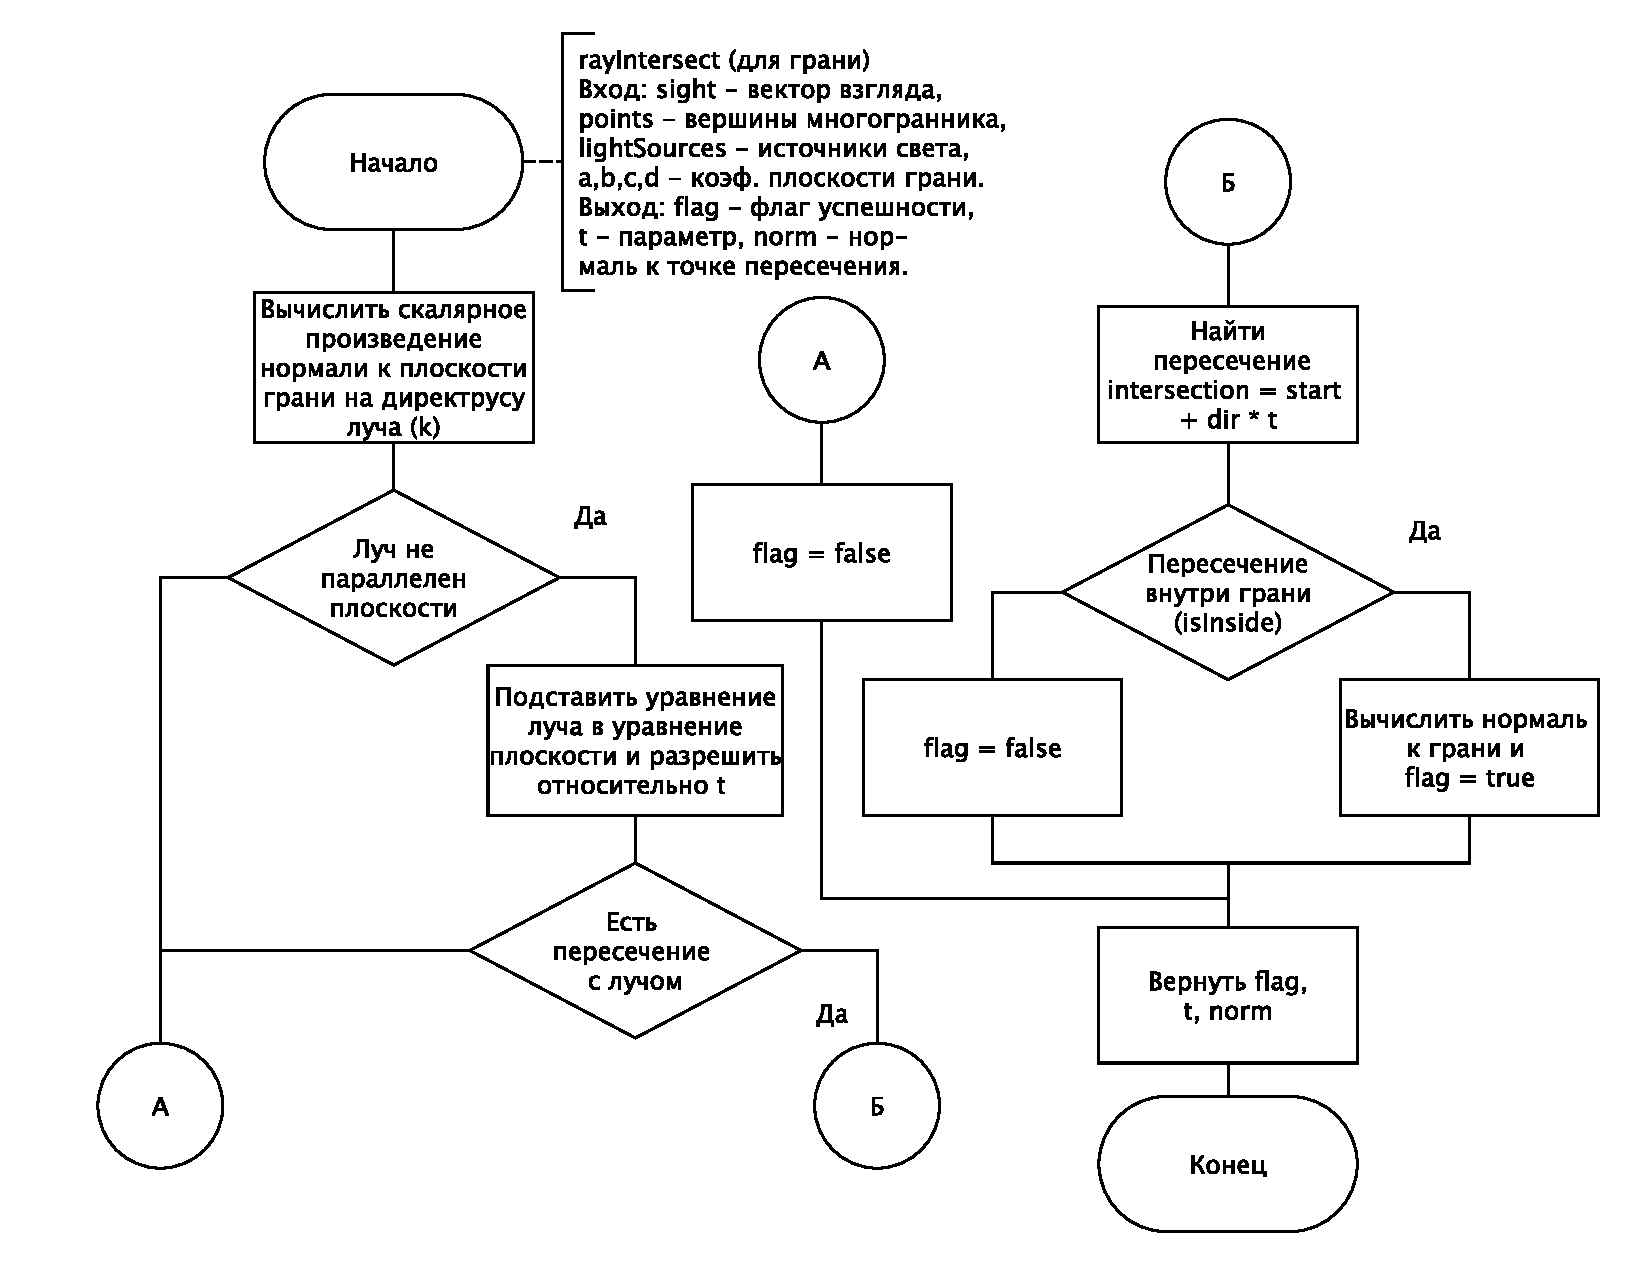
\includegraphics[width=0.75\linewidth]{rayGran.pdf}
    \caption{Схема подпрограммы поиска точки пересечения луча с треугольным полигоном}
    \label{img:rayGran}
\end{figure}

\newpage

На рисунке \ref{img:raySphere} представлена схема подпрограммы поиска точки пересечения луча со сферой.

\begin{figure}[h!]
    \centering
    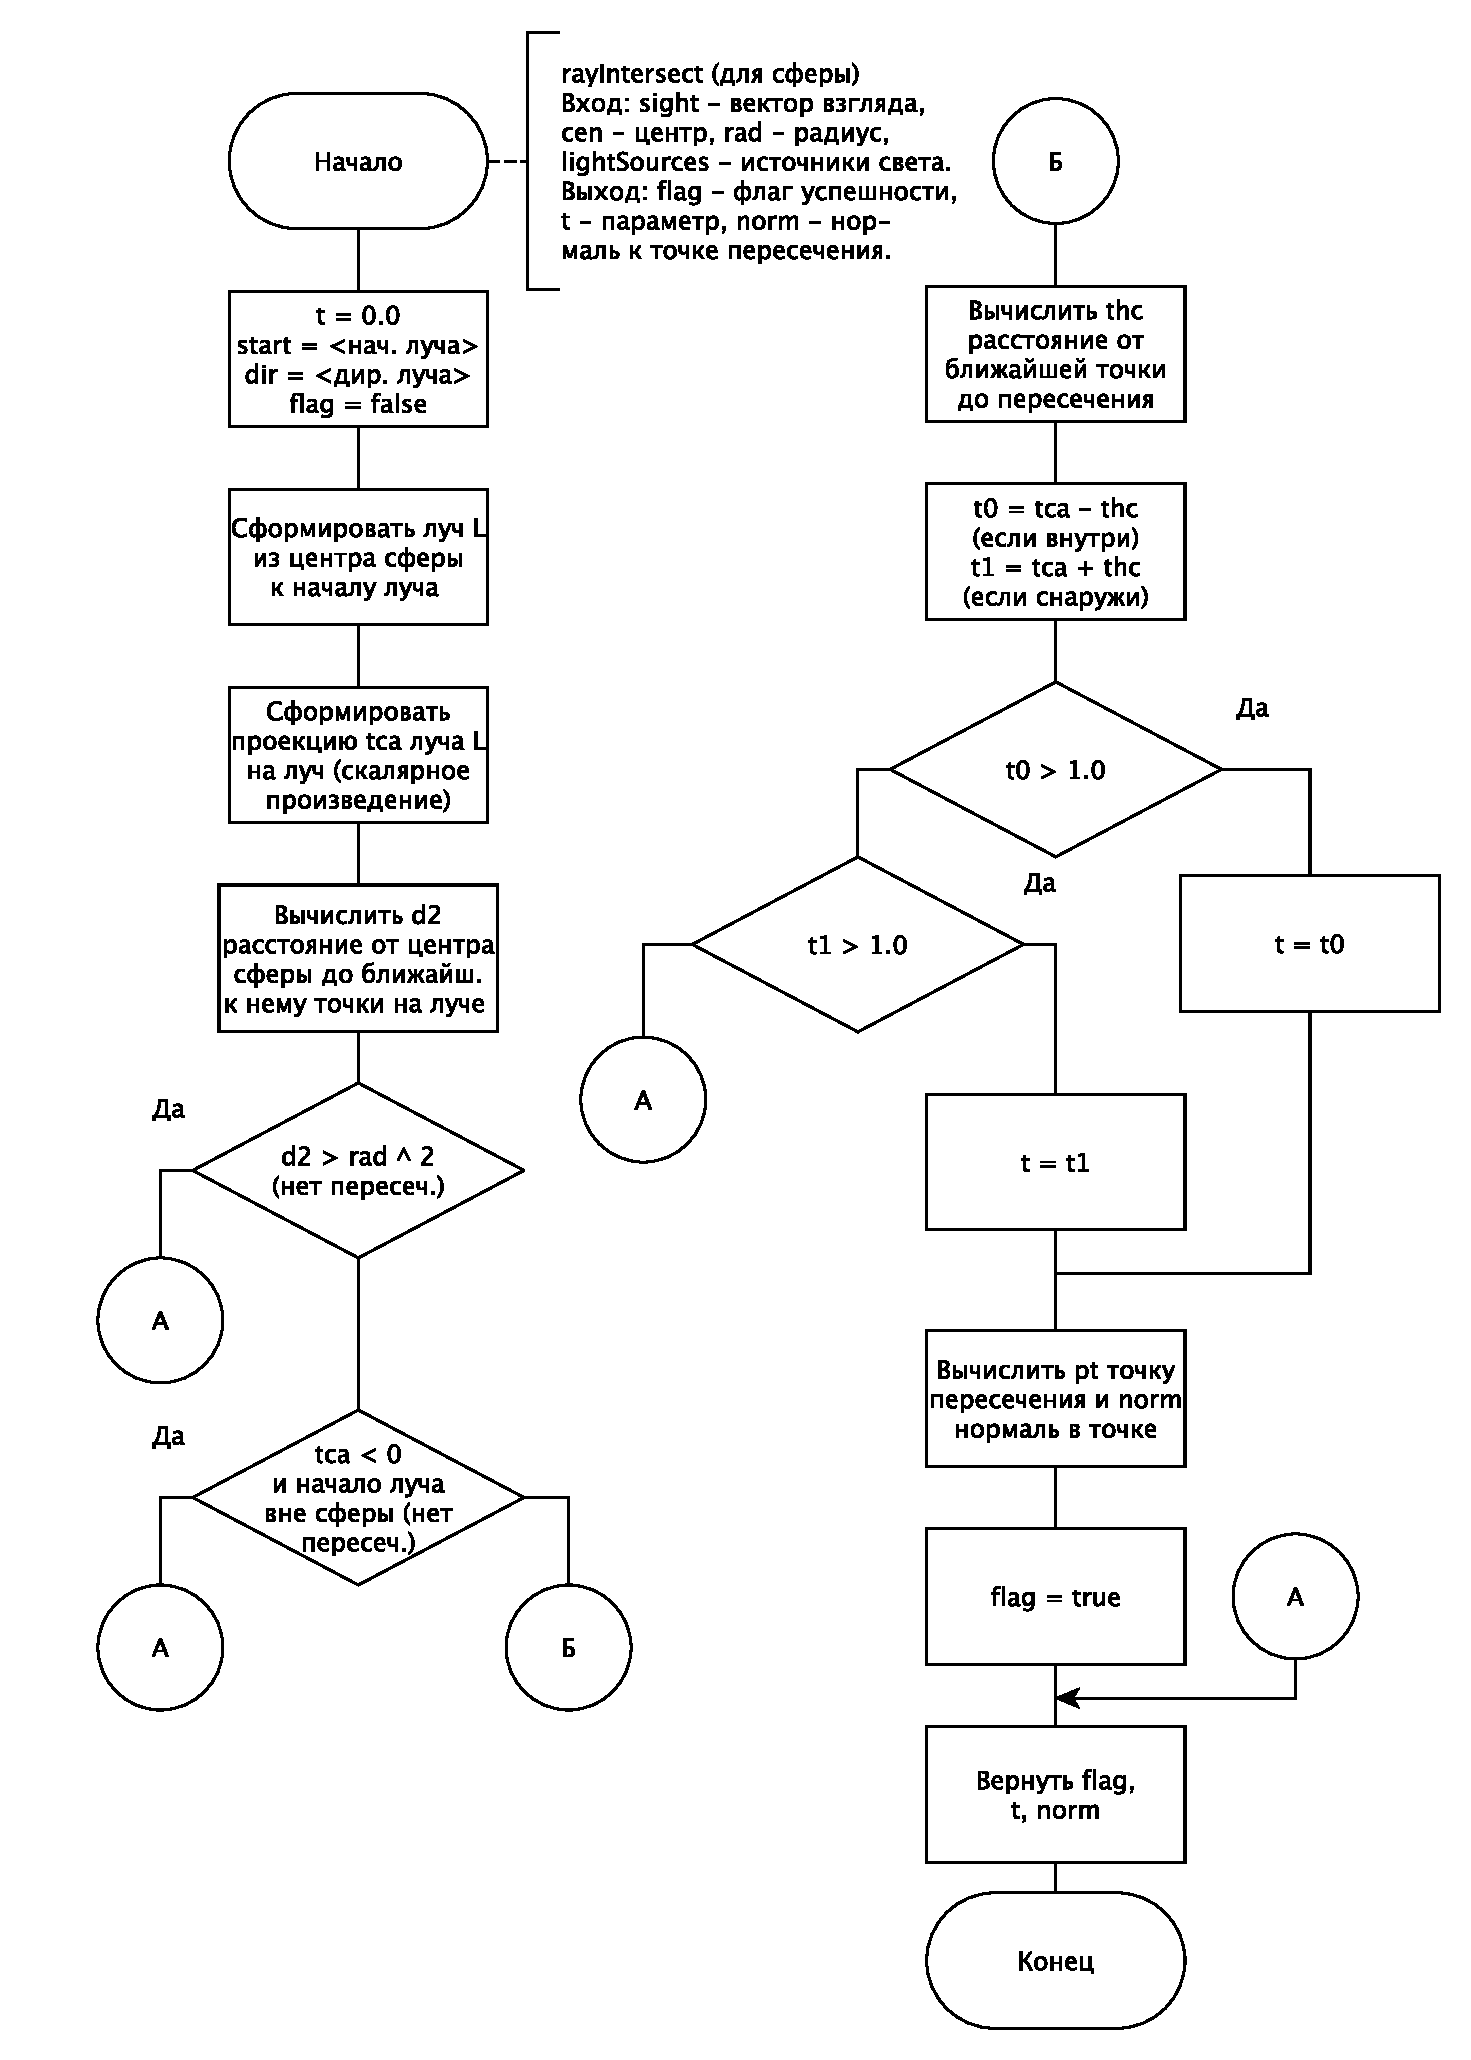
\includegraphics[width=0.85\linewidth]{raySphere.pdf}
    \caption{Схема подпрограммы поиска точки пересечения луча со сферой}
    \label{img:raySphere}
\end{figure}

\newpage

На рисунке \ref{img:isInside} представлена схема подпрограммы проверки принадлежности точки грани.

\begin{figure}[h!]
    \centering
    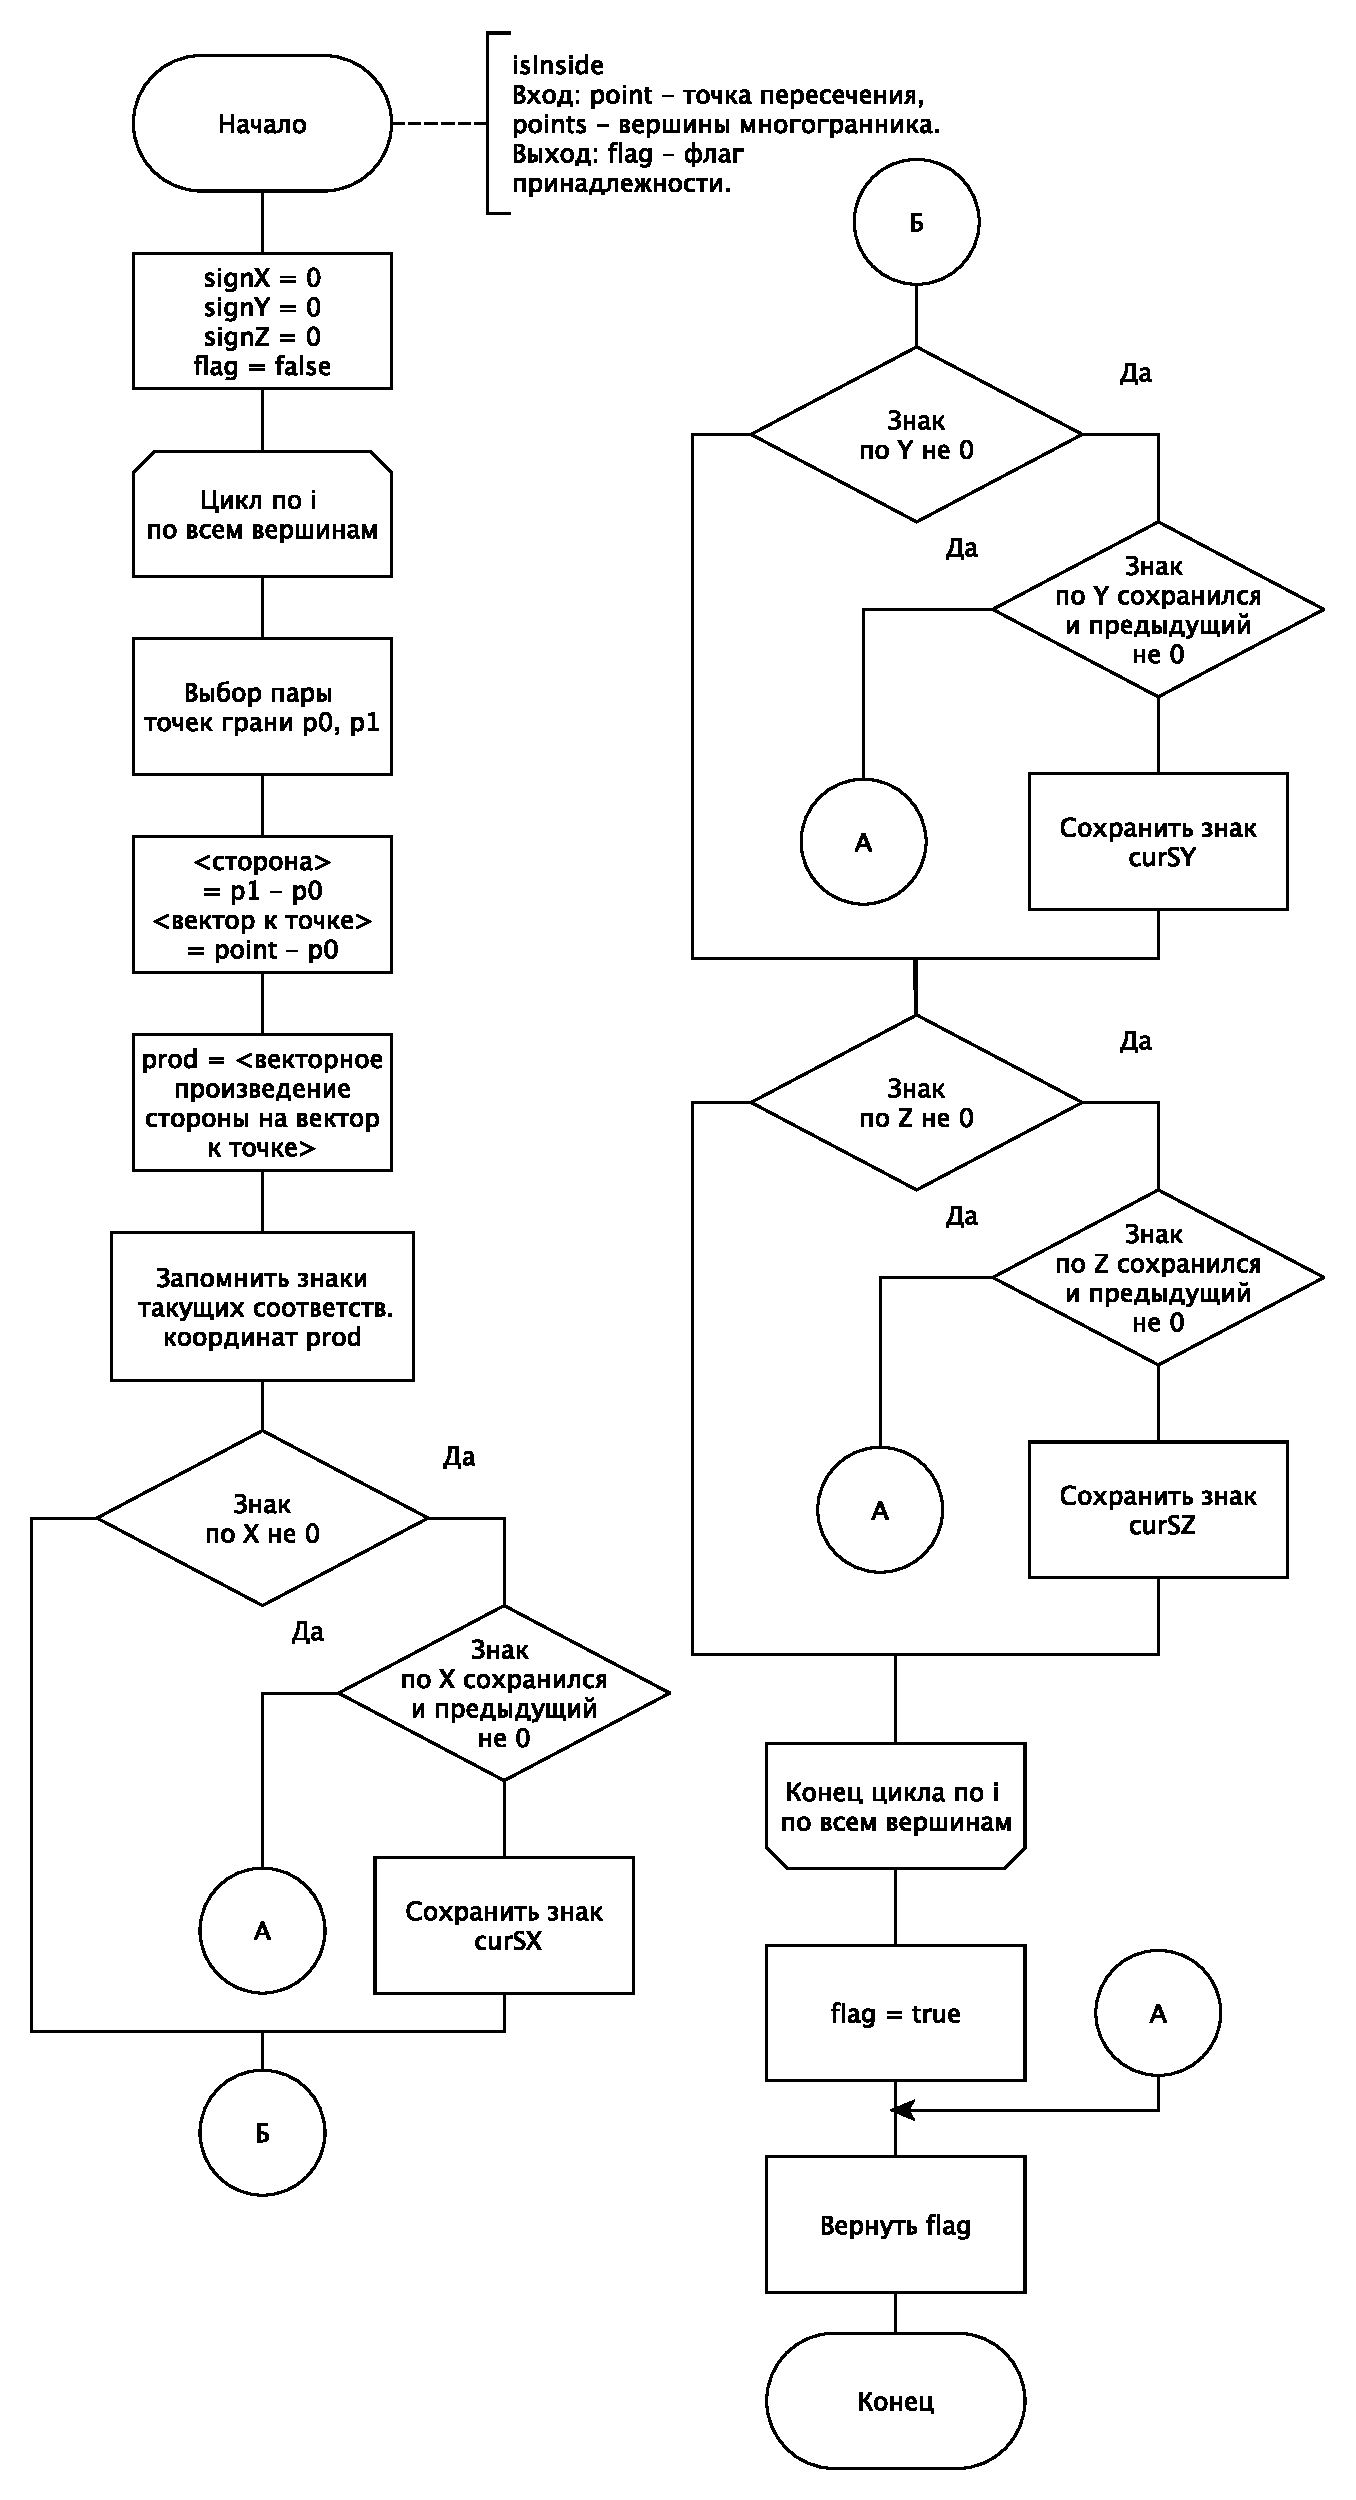
\includegraphics[width=0.65\linewidth]{isInside.pdf}
    \caption{Схема подпрограммы проверки принадлежности точки грани}
    \label{img:isInside}
\end{figure}

%\section{Разработка алгоритма однопоточной реализации обратной трассировки лучей}
%На рисунке \ref{img:one} представлена схема алгоритма однопоточной реализации обратной трассировки лучей.
%
%\begin{figure}[h!]
%    \centering
%    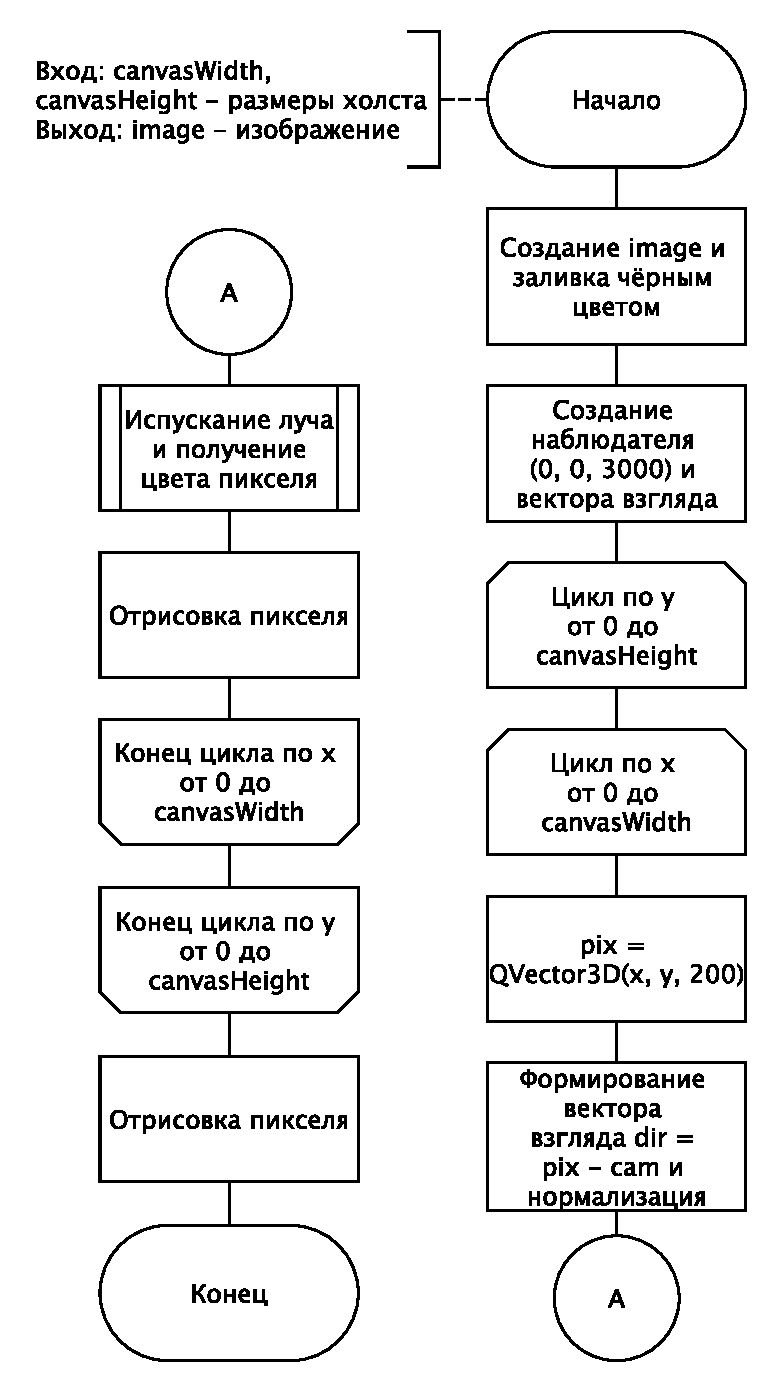
\includegraphics[width=0.6\linewidth]{one.pdf}
%    \caption{Схема алгоритма однопоточной реализации обратной трассировки лучей}
%    \label{img:one}
%\end{figure}
%
%\section{Разработка алгоритма многопоточной реализации обратной трассировки лучей}
%На рисунке \ref{img:many} представлена схема алгоритма многопоточной реализации обратной трассировки лучей.
%
%\begin{figure}[h!]
%    \centering
%    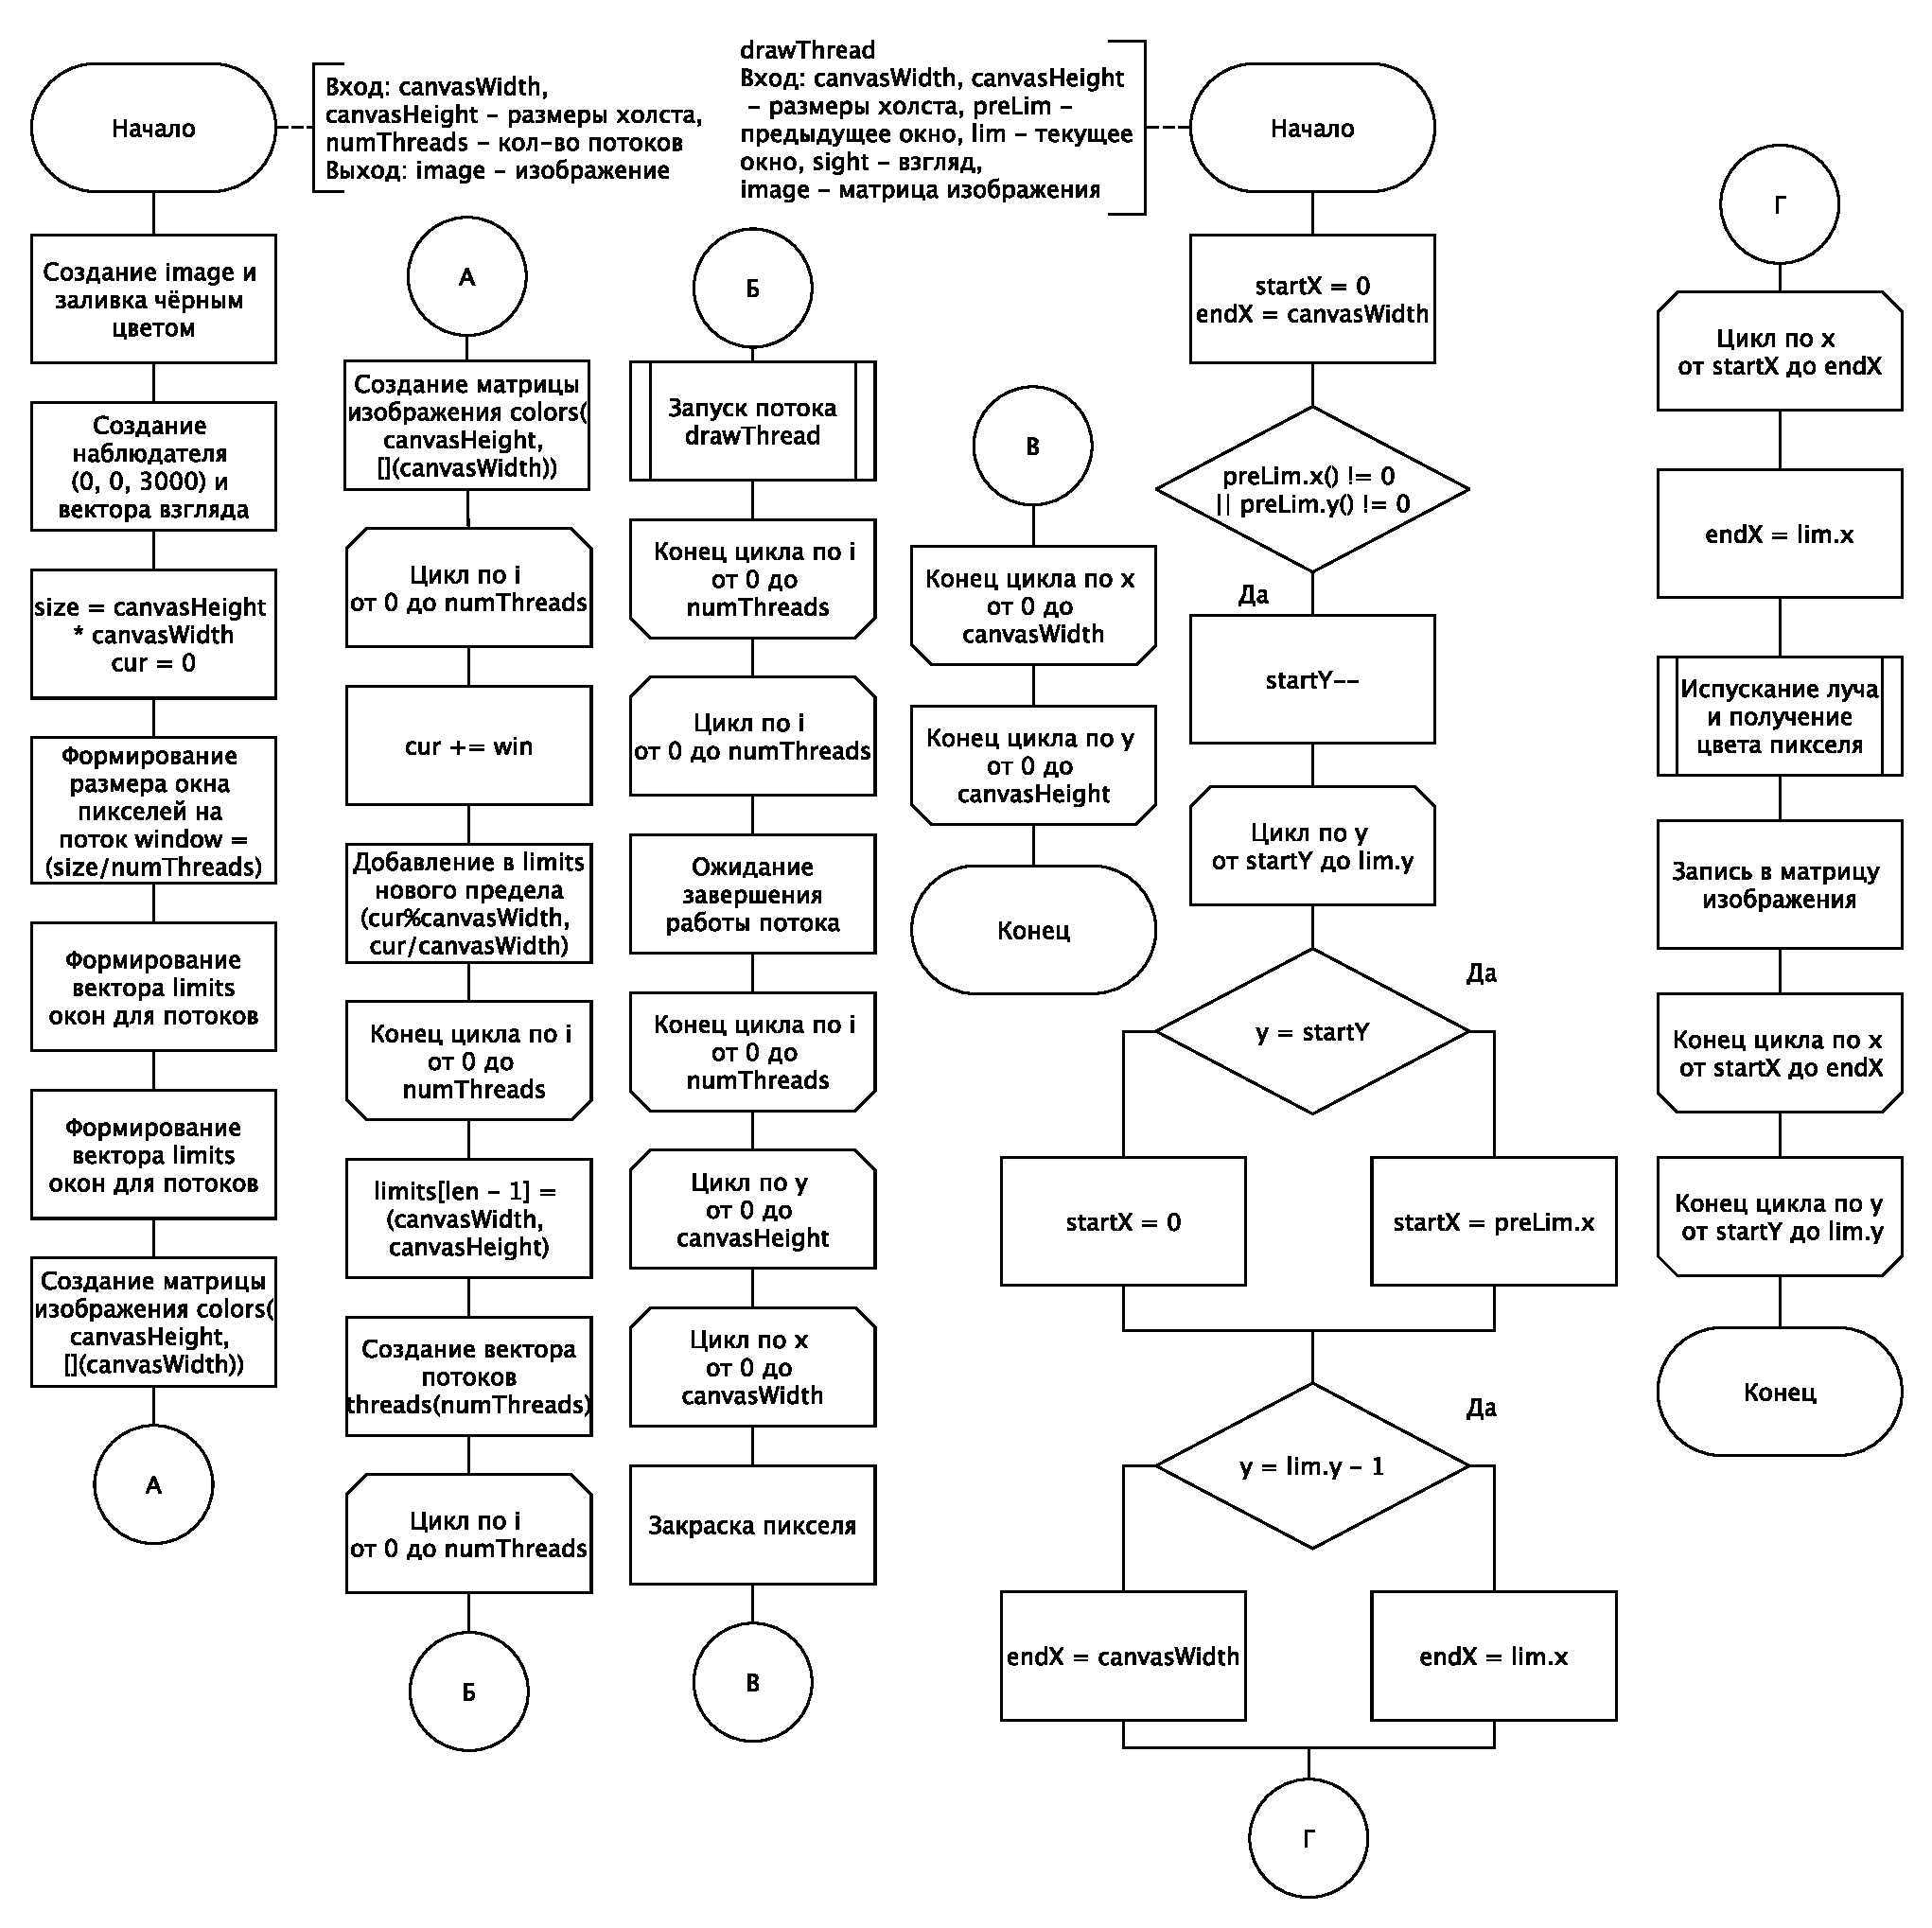
\includegraphics[width=1\linewidth]{many.pdf}
%    \caption{Схема алгоритма многопоточной реализации обратной трассировки лучей}
%    \label{img:many}
%\end{figure}

\section{Обоснование используемых типов и структур данных}
При реализации алгоритма обратной трассировки лучей для синтеза реалистичного изображения были использованы следующие типы и структуры данных:
\begin{enumerate}[label={\arabic*)}]
	\item Сцена ($drawing$) представляет из себя структуру со следующими полями: \begin{itemize}
		\item массив объектов сцены;
		\item камера (наблюдатель);
		\item массив источников света на сцене.
	    \end{itemize}
	Объекты сцены хранятся в массивах, для обеспечения доступа к отдельному объекту со сложностью $O(1)$ с помощью индексации и работы с итераторами. Объекты разного типа хранятся в разных массивах во избежание усложнённого выбора элементов.
	\item Объект-фигура ($figure$) представляет из себя структуру, содержащую поле с информацией о свойствах материала объекта типа $material$, описанного ниже.
	\item Многогранник ($polyhedron$) представляет из себя структуру со следующими полями: \begin{itemize}
		\item массив вершин;
		\item массив связей вершин (полигонов);
		\item сферическую оболочку типа $sphere$, описанного ниже.
	    \end{itemize}
	Элементы многогранника хранятся в массивах, для обеспечения доступа к отдельному объекту со сложностью $O(1)$ с помощью индексации и работы с итераторами. Сферическая оболочка необходима для ускорения проверки на пересечение многогранника лучом.
	\item Полигон ($polygon$) представляет из себя структуру со следующими полями: вектор вершин и набор коэффициентов задающей грань плоскости (для точности вычислений используется числовой тип двойной точности). Элементы полигона хранятся в массивах, для обеспечения доступа к отдельному объекту со сложностью $O(1)$ с помощью индексации и работы с итераторами.
	\item Сфера ($sphere$) представляет из себя структуру, содержащую поля с информацией о векторе радиуса и точке центра (координаты типа вектор).
	Это позволяет задавать сферу аналитическим образом для работы с программой.
	\item Источник света ($lightSource$) представляет из себя структуру, содержащую информацию о расположении источника в пространстве (координаты типа вектор) и числовое значение его интенсивности (для точности вычисления цвета используется числовой тип двойной точности). Структура источника света, если расположен в бесконечности, также хранит информацию о направлении распространения света (координаты типа вектор). Предусмотрен только белый цвет излучения.
	\item Камера ($camera$) представляет из себя структуру, содержащую поля с информацией о расположении наблюдателя в пространстве и направлении вектора его взгляда (координаты типа вектор).
	\item Материал ($material$) представляет из себя структуру со следующими полями: \begin{itemize}
		\item цвет фонового освещения (три целочисленных переменных в модели RGB);
		\item цвет диффузного освещения (три целочисленных переменных в модели RGB);
		\item цвет зеркального освещения (три целочисленных переменных в модели RGB);
		\item коэффициент фонового освещения (вещественная переменная двойной точности);
		\item коэффициент диффузного освещения (вещественная переменная двойной точности);
		\item коэффициент зеркального освещения (вещественная переменная двойной точности);
		\item степень, аппроксимирующая пространственное распределение зеркально отражённого света (целочисленная переменная);
		\item коэффициент отражения (вещественная переменная двойной точности);
		\item коэффициент преломления (вещественная переменная двойной точности);
		\item показатель преломления (вещественная переменная двойной точности).
	    \end{itemize}
	    Все данные, влияющие на цвет закраски пикселов изображения, хранятся с использованием типов с двойной точностью как наиболее важные для решения поставленных задач, требующих повышенную точность вычислений.
\end{enumerate}

%\section{Диаграмма классовой структуры проекта}
%На рисунке \ref{img:classes} представлена диаграмма классовой структуры проекта.
%
%\begin{figure}[h!]
%    \centering
%    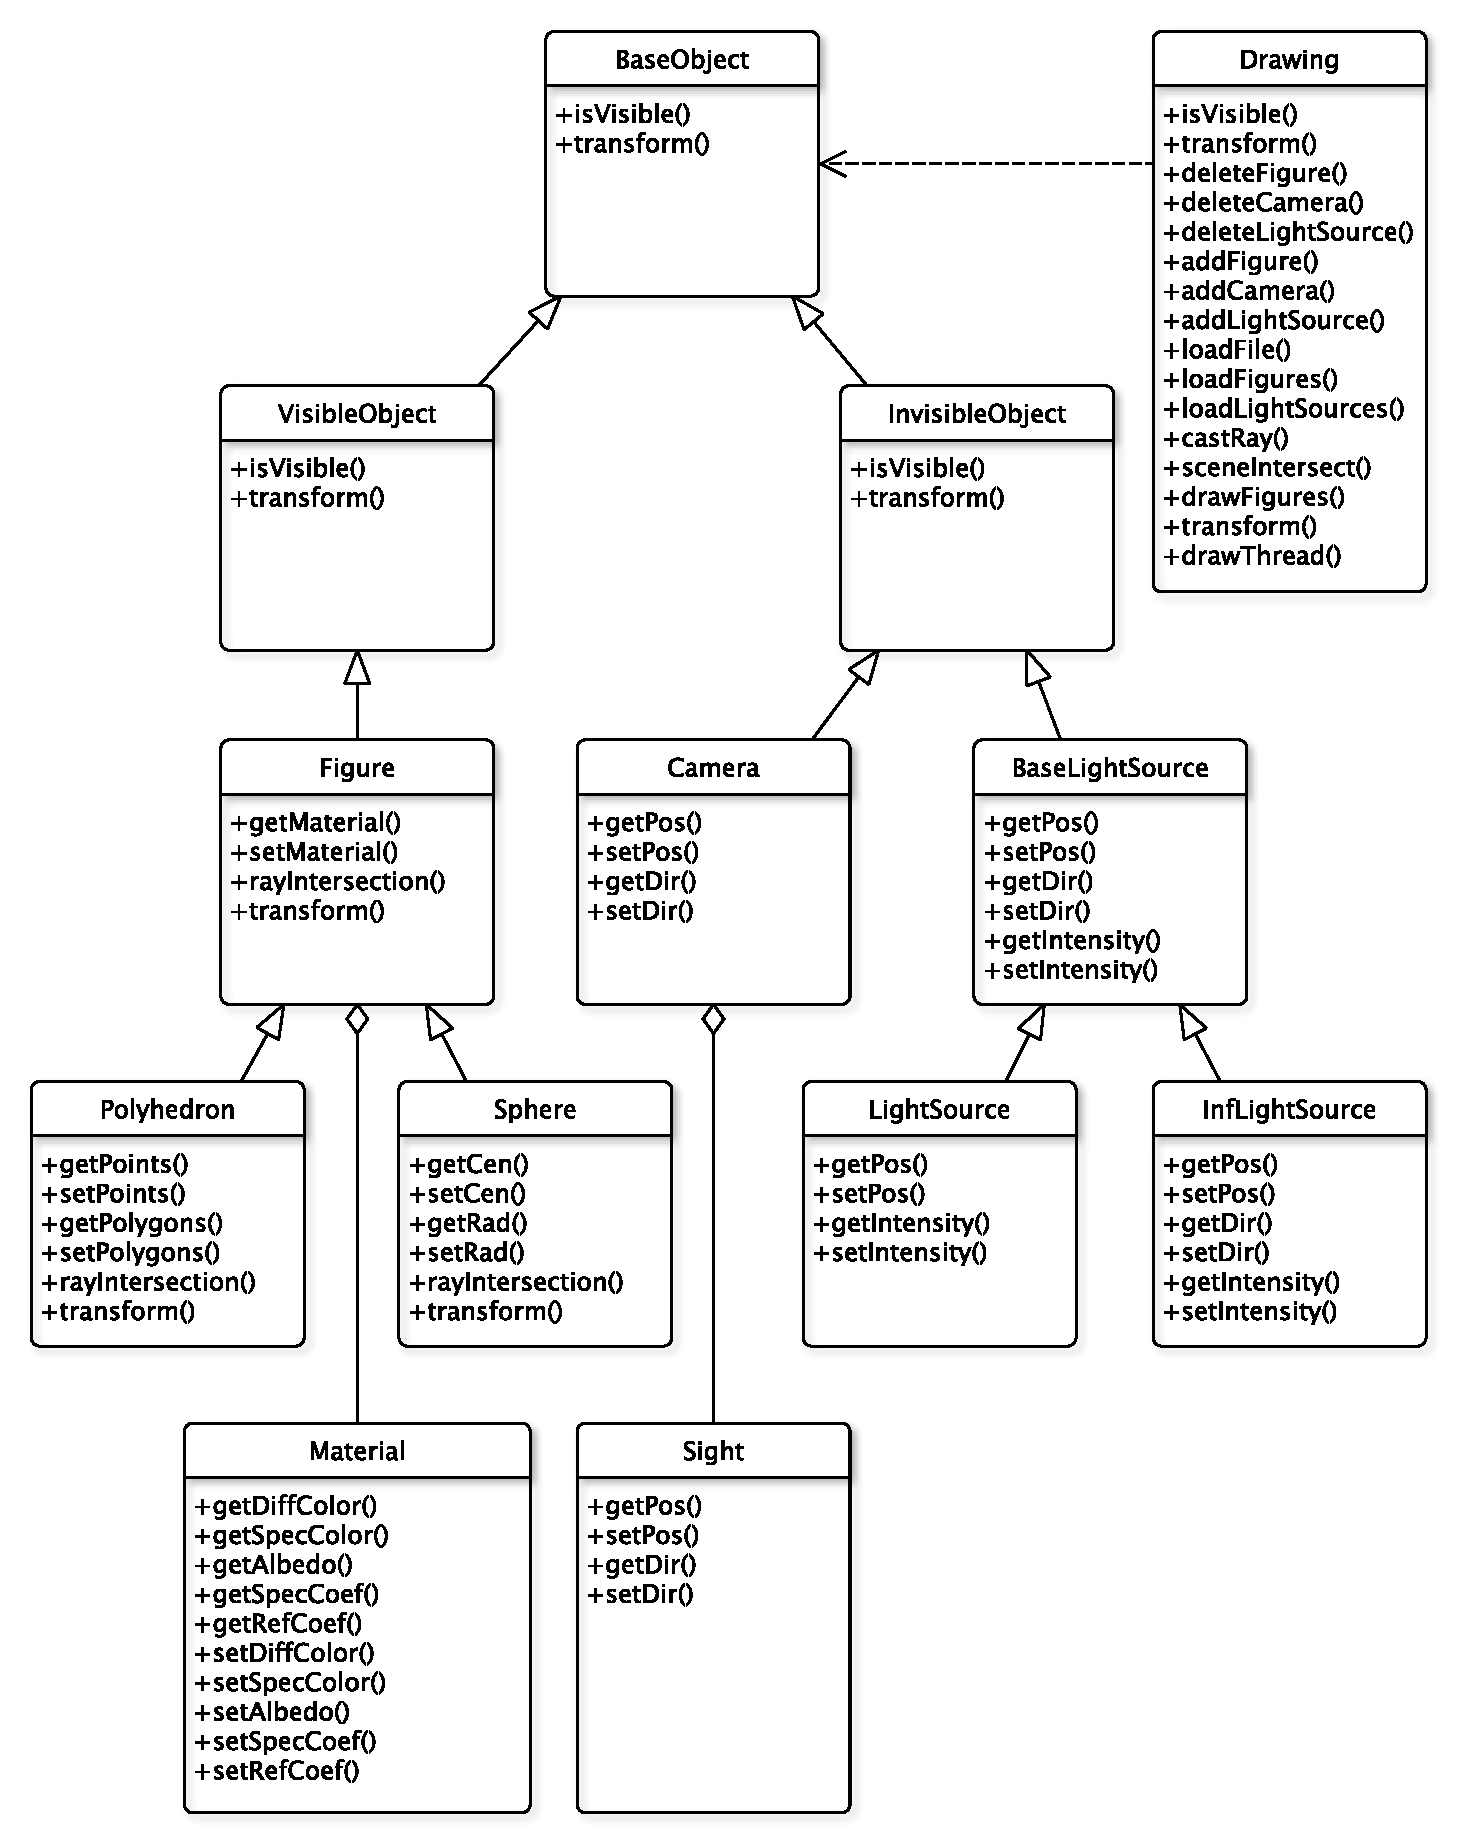
\includegraphics[width=0.8\linewidth]{classes.pdf}
%    \caption{Диаграмма классовой структуры проекта}
%    \label{img:classes}
%\end{figure}

\section{Выводы по конструкторской части}
В данном разделе были представлены математические основы для реализации алгоритма обратной трассировки лучей, схемы данного алгоритма и необходимых подпрограмм и обоснование используемых типов и структур данных.

\newpage